\documentclass{beamer}

\usepackage{beamerthemesplit}
\usetheme{Singapore}

\input{../../include/preamble.inc} 
\input{../../include/definitions.inc} 
\input{../../include/author.inc} 


\title[]{Cилы, действующие на сплошную среду, тензор напряжений}

\begin{document}
	
\frame[plain]{\titlepage}


\frame[plain]{
	\frametitle{Аннотация}
	\parbox{\textwidth}{
		Объемные и массовые силы. Поверхностные силы. Тензор напряжений Коши. Разложение напряжения на составляющие. Главные напряжения и оси тензора напряжений. 
	}
}

\frame{
	\frametitle{ Объемные и массовые силы }
	
	\begin{exampleblock}{Определение }
		\parbox{\textwidth}{
			Силы, действующие на каждый элемент объема $d\omega$ независимо от того, существуют ли рядом с объемом $d\omega$ другие частицы или нет, называются  \alert{объемными}. 	Если такие силы отнесены к единице массы, то они называются \alert{массовыми}.
		}
	\end{exampleblock}\pause

	\begin{exampleblock}{Пример}
		\parbox{\textwidth}{
		Объемная сила, действующая на частицу среды в поле силы тяжести, определяется соотношением:
		\[
		d\vec{F} = \rho \vec{g} d\omega,
		\]
		где $\rho$ -- плотность жидкой частицы; $\vec{g}$ -- вектор ускорения свободного падения.
		}
	\end{exampleblock}
}

\frame{
	\frametitle{ Поверхностные силы }
	
	\begin{columns}
		\begin{column}{0.35\textwidth}
			\parbox{\textwidth}{
				\centering
				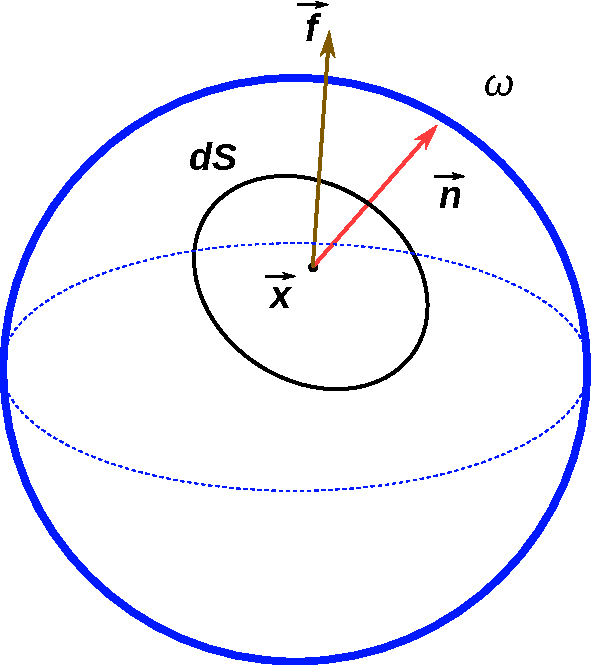
\includegraphics[width=\textwidth]{../img/sigma_def.pdf}
				
				\medskip	
				\scriptsize
				\parbox{\textwidth}{
				Выделенный объем сплошной среды $\omega$ с фиксированной точкой $\vec{x}$ внутри него и элементарной площадкой $dS$ с единичной нормалью $\vec{n}$		

				}

			}
		\end{column}
		\begin{column}{0.65\textwidth}
			\begin{exampleblock}{Определение }
				\parbox{\textwidth}{
					\alert{Напряжением поверхностной силы} $\vec{f}$ называется величина силы, отнесенная к элементарной площадке $dS$ с единичной нормалью $\vec{n}$, возникающая в результате взаимодействия частей среды с разных сторон от элементарной площадки в малой окрестности точки $\vec{x}$. 
				}
			\end{exampleblock}
		

		\end{column}
	\end{columns}
}

\frame{
	\frametitle{ Поверхностные силы  }
		\begin{columns}
		\begin{column}{0.35\textwidth}
			\parbox{\textwidth}{
				\centering
				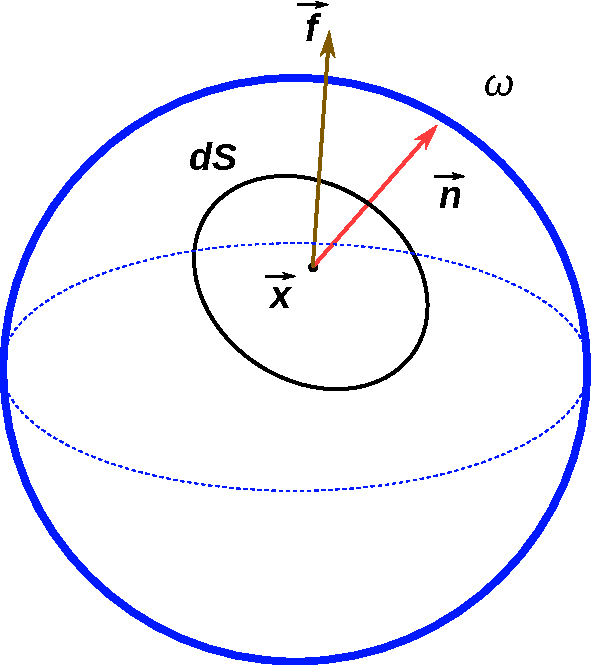
\includegraphics[width=\textwidth]{../img/sigma_def.pdf}
				
				\medskip	
				\scriptsize
				\parbox{\textwidth}{
					Выделенный объем сплошной среды $\omega$, с фиксированной точкой $\vec{x}$ внутри него и элементарной площадкой $dS$ с единичной нормалью $\vec{n}$					
				}
				
			}
		\end{column}
		\begin{column}{0.65\textwidth}
			
			\begin{exampleblock}{Замечания}
				\parbox{\textwidth}{
					\begin{enumerate}[partopsep=1pt,label=\arabic{enumi})]
						\item поверхностная сила существует в каждой точке среды (как на поверхности, так и на границе);
						\item поверхностная сила является функцией точки среды $\vec{x}$ и ориентации площадки  $\vec{n}$:
						\[
						\vec{f} = \vec{f}(\vec{x},\vec{n});
						\]
						\item считаем, что $\vec{n}$ -- вектор внешней единичной нормали;
					\end{enumerate}
				}
			\end{exampleblock}
		\end{column}
	\end{columns}
}


\frame{
	\frametitle{ Поверхностные силы  }
	\begin{columns}
		\begin{column}{0.35\textwidth}
			\smallskip
			\parbox{\textwidth}{
				\centering
				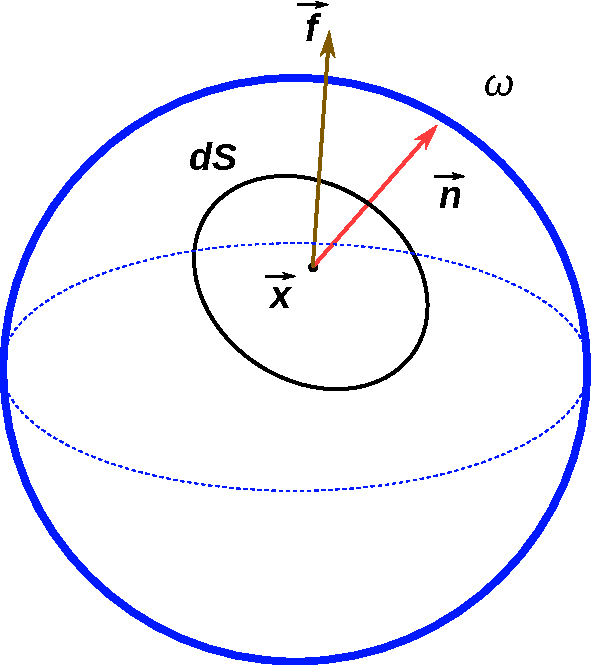
\includegraphics[width=\textwidth]{../img/sigma_def.pdf}
				
				\medskip	
				\scriptsize
				\parbox{\textwidth}{
					Выделенный объем сплошной среды $\omega$ с фиксированной точкой $\vec{x}$ внутри него и элементарной площадкой $dS$ с единичной нормалью $\vec{n}$					
				}
				
			}
		\end{column}
		\begin{column}{0.65\textwidth}
			
			\begin{exampleblock}{Замечания}
				\smallskip
				\parbox{\textwidth}{
					\begin{enumerate}[partopsep=1pt,label=\arabic{enumi}), start=4]
						\item для определения суммарной силы, действующей на объем $\omega$, ограниченный поверхностью $S$, необходимо проинтегрировать $\vec{f}(\vec{x},\vec{n}(\vec{x}))$ по этой поверхности:
						\[
						\vec{F} = \int\limits_{S}\vec{f}(\vec{x},\vec{n}(\vec{x}))dS.
						\]
					\end{enumerate}
				}
			\end{exampleblock}
		\end{column}
	\end{columns}
}





\frame{
	\frametitle{ Принцип равенства действий и противодействий  }
	
	\centering
	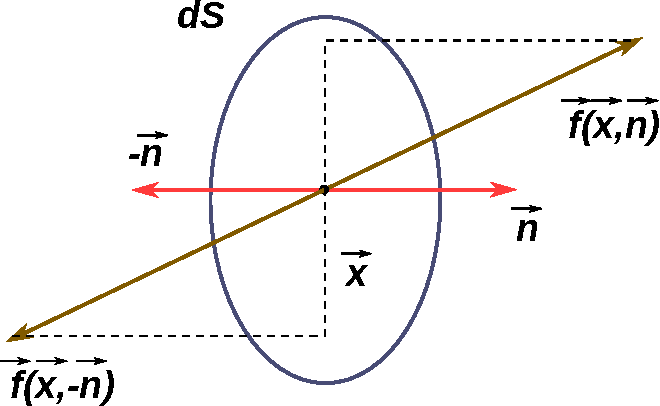
\includegraphics[width=0.5\textwidth]{../img/surface_action.pdf}\\
	{
		\scriptsize
		Иллюстрация равенства напряжения на противоположных направлениях		
	}	
	
	\bigskip
	\parbox{\textwidth}{
		Рассмотрим напряжения, возникающие в точке $\vec{x}$ на площадке с единичной нормалью $\vec{n}$ и ей противоположной, и вследствие принципа равенства действия и противодействия получим:
		\[
		\vec{f}(\vec{x},\vec{n}) = -\vec{f}(\vec{x},-\vec{n}).
		\]		
	}
}

\frame{
	\frametitle{ Тензор напряжений }
	
	
	\begin{columns}
		\begin{column}{0.5\textwidth}
			\centering
			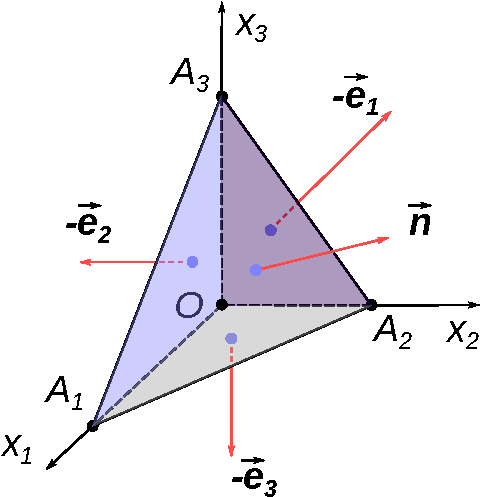
\includegraphics[width=\textwidth]{../img/cauchy_stress_tensor.pdf}
		\end{column}
		\begin{column}{0.5\textwidth}
			\parbox{\textwidth}{
			Выделим в сплошной среде в окрестности точки $O$ тетраэдр $OA_1A_2A_3$, у которого ребра $OA_1$, $OA_2$, $OA_3$ направлены вдоль координатных линий $x_1$, $x_2$, $x_3$, а грань $A_1A_2A_3$ перпендикулярна единичному вектору:
			\[
			\vec{n} =n^1 \vec{e}_1 + n^2 \vec{e}_2 + n^3 \vec{e}_3,
			\]
			\[
			|\vec{n}|=1.
			\]
			}
			

		\end{column}
	\end{columns}
}

\frame{
	\frametitle{ Тензор напряжений }
	
		\begin{columns}
		\begin{column}{0.4\textwidth}
			\centering
			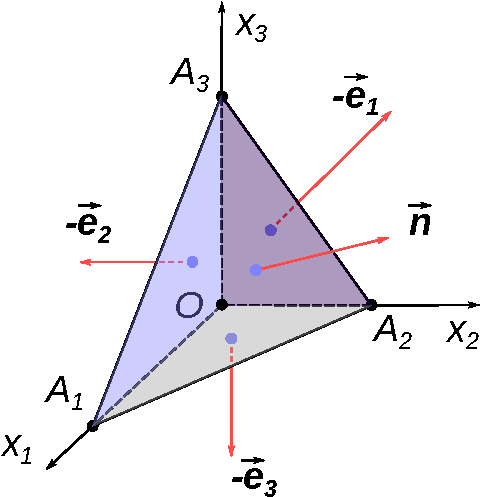
\includegraphics[width=\textwidth]{../img/cauchy_stress_tensor.pdf}
		\end{column}
		\begin{column}{0.6\textwidth}

			\begin{exampleblock}{Площади граней}
			\parbox{\textwidth}{
				\[
				\begin{array}{ccccc}
				S_1 & = & S_n \cos(\vec{n},\vec{e}_1) & = & S_n n^1,\\
				S_2 & = & S_n \cos(\vec{n},\vec{e}_2) & = & S_n n^2,\\
				S_3 & = & S_n \cos(\vec{n},\vec{e}_3) & = & S_n n^3,
				\end{array}
				\]
				где $S_i$, $S_n$ -- площади граней, ортогональных $\vec{e}_i$ ($i=1,2,3$) и $\vec{n}$. 
			}
			\end{exampleblock}
		
			\begin{exampleblock}{Объем тетраэдра}
				\parbox{\textwidth}{
					\[
					V = 1/3 S_n h,
					\]
					где $h$ -- длина перпендикуляра, опущенного из точки $O$ на грань $A_1A_2A_3$.
				}
			\end{exampleblock}

			
			
		\end{column}
	\end{columns}
	
}

\frame{
	\frametitle{Тензор напряжений }
	
	\begin{columns}
		\begin{column}{0.4\textwidth}
		\centering
		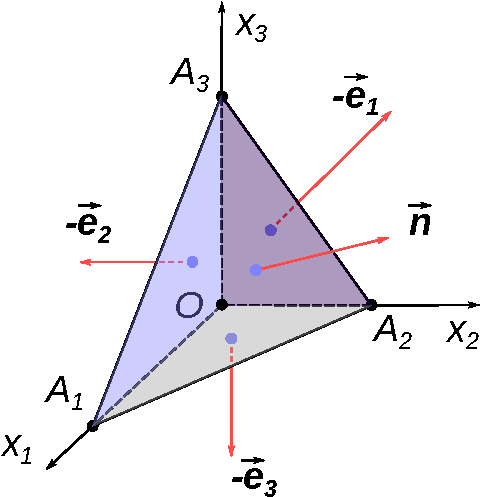
\includegraphics[width=\textwidth]{../img/cauchy_stress_tensor.pdf}
		\end{column}
		\begin{column}{0.6\textwidth}
			\begin{exampleblock}{Уравнения равновесия поверхностных сил в точке}
				\medskip
				\parbox{\textwidth}{
					
					\[
					\int\limits_V\vec{\Phi} dV + \int\limits_S\vec{f}(\vec{x},\vec{n}(\vec{x}))dS = 0 
					\]
					\[
					(\vec{\Phi} = \rho(\vec{F}-\vec{a})),
					\]
					где $\vec{\Phi}$ -- отнесенная к единице объема сумма внешних объемных сил $\vec{F}$ и сил инерции из-за ускорения $\vec{a}$ -- материальных точек.					
				}
			\end{exampleblock}
		\end{column}
	\end{columns}
	
}

\frame{
	\frametitle{ Тензор напряжений }
	
	\begin{exampleblock}{Оценка объемного интеграла для уравнения равновесия}
		\parbox{\textwidth}{
			По теореме о среднем:
			\[
			\int\limits_V\vec{\Phi} dV = \vec{\Phi}(M)V = \frac{1}{3}  \vec{\Phi}(M)S_n h ,
			\]
			где $M$ -- точка внутри тетраэдра; $V$ -- объем тетраэдра.
		}
	\end{exampleblock}
	

	
}

\frame{
	\frametitle{Тензор напряжений }
	
	\begin{exampleblock}{Разложение }
		\parbox{\textwidth}{
			Используя принцип равенства действий и противодействий, имеем:
			\[
			\int\limits_S\vec{f}(\vec{x},\vec{n}(\vec{x}))dS = 		\int\limits_{S_1}\vec{f}(\vec{x},-\vec{e}_1)dS +
			\int\limits_{S_2}\vec{f}(\vec{x},-\vec{e}_2)dS +		
			\int\limits_{S_3}\vec{f}(\vec{x},-\vec{e}_3)dS +
			\]
			\[			
			+\int\limits_{S_n}\vec{f}(\vec{x},\vec{n})dS =	\pause
			-\int\limits_{S_1}\vec{f}(\vec{x},\vec{e}_1)dS -
 	    	\int\limits_{S_2}\vec{f}(\vec{x},\vec{e}_2)dS -		
			\int\limits_{S_3}\vec{f}(\vec{x},\vec{e}_3)dS +
			\]
			\[
			+ \int\limits_{S_n}\vec{f}(\vec{x},\vec{n})dS =
			\]
		}
	\end{exampleblock}
	
}

\frame{
	\frametitle{ Тензор напряжений  }
	
	\begin{exampleblock}{Оценка поверхностного интеграла}
		
		\parbox{\textwidth}{
		По теореме о среднем для поверхностного интеграла  существуют точки $M_i$ и $M_n$  на поверхностях $S_i$ ($i=1,2,3$) и $S_n$ такие, что
		\[
		= -S_1 \vec{f}(M_1,\vec{e}_1) -
		  S_2 \vec{f}(M_2,\vec{e}_2) -		
		  S_3 \vec{f}(M_3,\vec{e}_3) +
		  S_n\vec{f}(M_n,\vec{n}) =
		\]	\pause 
		Используя связь площадей боковых граней пирамиды тетраэдра и ее основания, получаем:
		\[
			= -S_n (\vec{f}(M_1,\vec{e}_1) n^1 +
					\vec{f}(M_2,\vec{e}_2) n^2 +		
					\vec{f}(M_3,\vec{e}_3) n^3 -
					\vec{f}(M_n,\vec{n})).
		\]	
		
			
		}
	\end{exampleblock}
	
}

\frame{
	\frametitle{ Тензор напряжений }
	
	\begin{exampleblock}{Формула для напряжения на произвольной площадке}
		\parbox{\textwidth}{
			Таким образом, сокращая на $S_n$, имеем:
			\[
			 -\frac{1}{3}  \vec{\Phi}(M) h =  \vec{f}(M_1,\vec{e}_1) n^1 +
			 \vec{f}(M_2,\vec{e}_2) n^2 +		
			 \vec{f}(M_3,\vec{e}_3) n^3 -
			 \vec{f}(M_n,\vec{n}).
			\]\pause
			При $h \to 0$ точки $M_i \to O$, $M_n \to O$, $M \to O$, при этом левая часть равенства стремится к $0$. \pause
			
			\medskip			
			Таким образом,  для произвольной точки $O$: \alert{
			\[
				\vec{f}(O,\vec{n}) = \vec{f}(O,\vec{e}_1) n^1 +
				\vec{f}(O,\vec{e}_2) n^2 +		
				\vec{f}(O,\vec{e}_3) n^3.
			\]}
			
		}
	\end{exampleblock}
	
}

\frame{
	\frametitle{ Тензор напряжений }
	

	
	\begin{columns}
		\begin{column}{0.45\textwidth}
			\centering
			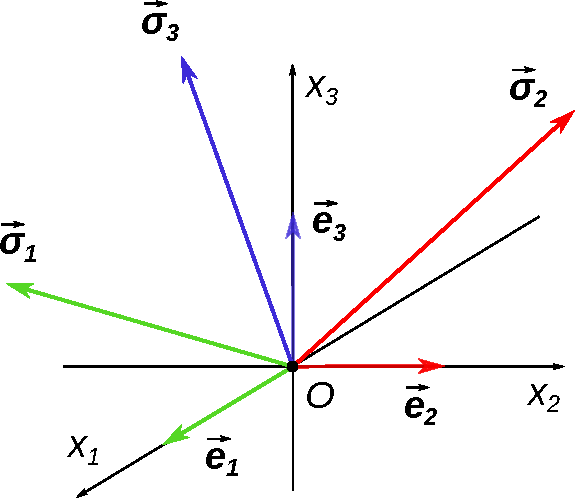
\includegraphics[width=\textwidth]{../img/sigmai_wp.pdf}
		\end{column}
		\begin{column}{0.55\textwidth}
			\parbox{\textwidth}{
				Напряжение в точке $\vec{x}$ на площадке, перпендикулярной $\vec{n}$, вычисляется по формуле:
			\alert{
				\[
				\vec{f}(\vec{x},\vec{n}) = \vec{\sigma}_n(\vec{x}) =  n^i \vec{\sigma_i}(\vec{x})=n^i \sigma_i^j(\vec{x})\vec{e}_j,
				\]	
				\[
				|\vec{n}|=1.
				\]
			}
			}
		\end{column}
	\end{columns}
	
	
	\begin{exampleblock}{Обозначения}
		\parbox{\textwidth}{
			\begin{eqnarray*}
				\vec{f}(\vec{x},\vec{e}_1) & = & \sigma_1^1 (\vec{x})\vec{e}_1 +  \sigma_1^2 (\vec{x})\vec{e}_2 +  \sigma_1^3 (\vec{x})\vec{e}_3 = \vec{\sigma}_1(\vec{x}), \\
				\vec{f}(\vec{x},\vec{e}_2) & = & \sigma_2^1 (\vec{x})\vec{e}_1 +  \sigma_2^2 (\vec{x})\vec{e}_2 +  \sigma_2^3 (\vec{x})\vec{e}_3 = \vec{\sigma}_2(\vec{x}), \\
				\vec{f}(\vec{x},\vec{e}_3) & = & \sigma_3^1 (\vec{x})\vec{e}_1 +  \sigma_3^2 (\vec{x})\vec{e}_2 +  \sigma_3^3 (\vec{x})\vec{e}_3 = \vec{\sigma}_3(\vec{x}).
			\end{eqnarray*}
			}
		
		
	\end{exampleblock}
}

\frame{
	\frametitle{ Тензор напряжений }
	
	\begin{exampleblock}{Определение нового базиса}
		\parbox{\textwidth}{
			Рассмотрим новый базис $\vec{g}_1$, $\vec{g}_2$, $\vec{g}_3$ в заданной точке такой, что
			\[
				\vec{e}_i  = \alpha_{i}^j \vec{g}_j,\quad
				\vec{g}_l  = \beta_l^j \vec{e}_j,
			\]
			где $\alpha_i^j$, $\beta_j^l$ -- матрицы перехода между базисами, причем $|\alpha_i^j|\neq 0$, $|\beta_j^l|\neq 0$ и $\alpha_i^j\beta_j^l=\delta_i^l$.
		}
	\end{exampleblock}
	\begin{exampleblock}{Формулы перехода}
		\parbox{\textwidth}{
			
			\[
				\vec{n} = \bar{n}^i \vec{g}_i = \bar{n}_i \beta_i^k \vec{e}_k= n^k \vec{e}_k
		 	\]
			Следовательно,  $n^k = \bar{n}^i \beta_i^k$.
			
			Тогда
			\[
				\vec{\sigma}_n = n^i \sigma_i^j \vec{e}_j = 
				\bar{n}^k \beta_k^i  \sigma_i^j \alpha_j^l\vec{g}_l =
				\bar{n}^k \bar{\sigma}_k^l \vec{g}_l,
%				
%							
%				= n_k' \alpha_{ik} \sigma_{ij}  =
			\]
			где $\bar{\sigma}_k^l = \beta_k^i \alpha_j^l \sigma_i^j$.  \alert{Такое преобразование компонентов матрицы $\sigma_{ij}$ является признаком смешанного тензора 2-го ранга.}
			
			
		}
	\end{exampleblock}	
}

\frame{
	\frametitle{Разложение напряжения}
	
	\begin{columns}
		\begin{column}{0.5\textwidth}
			\centering
			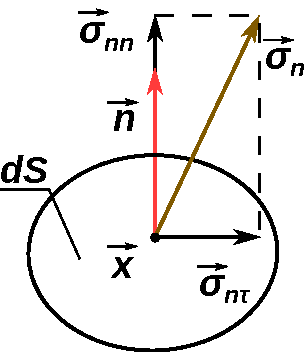
\includegraphics[width=0.7\textwidth]{../img/sigma_decomposition.pdf}
			
			\scriptsize
			Разложение напряжения на нормальную и тангенциальную составляющие
		\end{column}
		\begin{column}{0.5\textwidth}
			\parbox{\textwidth}{
				Напряжение в точке $\vec{x}$, возникающее на площадке $dS$ с единичной нормалью $\vec{n}$, можно представить в виде суммы нормальной $\vec{f}_n$ и тангенциальной составляющих $\vec{f}_\tau$:
				\[
				\vec{\sigma}_n = \vec{\sigma}_{nn}+\vec{\sigma}_{n\tau}.
				\]
				
				В этом случае $\vec{\sigma}_{nn}$ называется \alert{нормальным растяжением}, или \alert{нормальным давлением}. $\vec{\sigma}_{n\tau}$ называют \alert{косым напряжением}, или \alert{силой трения}.
			}
		\end{column}
	\end{columns}
	
}

\frame{
	\frametitle{ Выражения для нормальной и тангенциальной составляющих }
	\begin{columns}
	\begin{column}{0.4\textwidth}
		\centering
		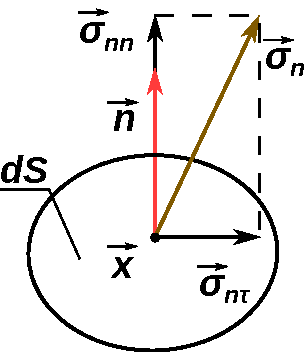
\includegraphics[width=0.7\textwidth]{../img/sigma_decomposition.pdf}
		
		\scriptsize
		Разложение напряжения на нормальную и тангенциальную составляющие
	\end{column}
	\begin{column}{0.6\textwidth}
		\begin{exampleblock}{Нормальная составляющая}
			\parbox{\textwidth}{
			\[
			\sigma_{nn} = \vec{\sigma}_n \cdot \vec{n}  = (n^i \sigma_i^j \vec{e}_j)\cdot (n^k \vec{e}_k) = 
			\]
			\[=
			n^i n^k \sigma_i^j (\vec{e}_j\cdot \vec{e}_k)=
			n^i n^k \sigma_{ik}
			\]				
			}
		\end{exampleblock}\pause
		\begin{exampleblock}{Тангенциальная составляющая}
			\parbox{\textwidth}{
			\[
			\sigma_{n\tau}^2 = \sigma_n^2-\sigma_{nn}^2  = 
			\]
			\[
			=
			(n^i \sigma_i^j \vec{e}_j)\cdot(n^k \sigma_k^l \vec{e}_l)-
			n^i n^j \sigma_{ij} n^k n^l \sigma_{kl} =
			\]
			\[
			= 
			n^i n^k \sigma_i^j \sigma_k^l (\vec{e}_j\cdot \vec{e}_l)  - 
			n^i n^j n^k n^l \sigma_{ij} \sigma_{kl}=
			\]
			\[
				=
				n^i n^k \sigma_{il} \sigma_{ks} g^{ls} - n^i n^j n^k n^l \sigma_{ij} \sigma_{kl}=
			\]
			\[\alert{
			=  n^i n^k \sigma_{il} \sigma_{ks} (g^{ls} - n^l n^s)
				}
			\]
			}
		\end{exampleblock}

	\end{column}
\end{columns}
}


\frame{
	\frametitle{ Главные напряжения, оси тензора напряжений }
	 
	 \begin{exampleblock}{Допущение}
	 	\parbox{\textwidth}{
	 		Будем считать, что тензор напряжений симметричный (в дальнейшем это утверждение будет обосновано):
	 		\[
	 		\sigma_{ij} = \sigma_{ji}.
	 		\]
	 	}
	 \end{exampleblock}
	 
	\begin{exampleblock}{Теорема о разложении}
		\parbox{\textwidth}{
			Для тензора напряжений в каждой точке сплошной среды сущест\-вует ортонормированная система координат, в которой он имеет диагональный вид, и имеются три направления, в которых дейст\-вуют только нормальные напряжения.
		}
	\end{exampleblock}
}

%\frame{
%	\frametitle{ Определение собственных векторов }
%	
%	\centering
%	
%	\alert{
%		\Huge
%		Вывод диагональности тензора в системе координат собственных векторов
%	}
%}



\frame{
	\frametitle{ Напряжение в системе координат главных осей}
	
	\begin{exampleblock}{}
		\parbox{\textwidth}{
		\small
		Пусть главные оси задаются ортонормированными векторами $\vec{g}_i$, а главные значения в этих осях тензора напряжений  $\sigma_i^j$ равны $\sigma_l$, тогда матрица перехода между ортонормированным базисом пространства $\vec{e}_j$ и введенным базисом будет ортогональная (обратная совпадает с транспонированной), т.е. 
		$
		\alpha_i^j \alpha^k_j = \delta_i^k,
		$
		а контравариантные, ковариантные и смешанные компоненты тензора совпадают.
		
		\medskip
		Напряжение на площадке с нормалью $\vec{n}$ имеет вид:	
		\[			
		\vec{\sigma}_n	= n^i\sigma_i^j \vec{e}_j = \bar{n}^k \bar{\sigma}_k^l  \vec{g}_l = 
		(\bar{n}^l \sigma_l) \vec{g}_l,
		\]
		где $\bar{n}^k$ -- координаты нормали в базисе $\vec{g}_k$;  $\bar{\sigma}_k^l = \sigma_k \delta_k^l$ -- тензор напряжений в главных осях.
		
		\medskip
		Таким образом, учитывая, что $|\vec{n}|=1$, из полученной формулы видим, что  вдоль главных осей имеют место только растягивающие или сжимающие напряжения.
		}
	\end{exampleblock}
	
}
\frame{
	\frametitle{Инварианты тензора напряжений}
	
	\begin{exampleblock}{Первый инвариант}
		\parbox{\textwidth}{
			
			\[
			I_1 = \operatorname{tr} \sigma = \sigma_1^1+\sigma_2^2+\sigma_3^3=\sigma_{1}+\sigma_2+\sigma_3,
			\]
			
			
		}
	\end{exampleblock}

	\begin{exampleblock}{Второй инвариант}
		\parbox{\textwidth}{
			\[
			I_2 = 
			\left|
			\begin{array}{cc}
			\sigma_1^1 & \sigma_1^2 \\
			\sigma_2^1 & \sigma_2^2
			\end{array}
			\right|+
			\left|
			\begin{array}{cc}
			\sigma_1^1 & \sigma_1^3 \\
			\sigma_3^1 & \sigma_3^3
			\end{array}
			\right|+
			\left|
			\begin{array}{cc}
			\sigma_2^2 & \sigma_2^3 \\
			\sigma_3^2 & \sigma_3^3
			\end{array}
			\right| = \sigma_1\sigma_2+\sigma_2\sigma_3+\sigma_1\sigma_3,
			\]
			
		}
	\end{exampleblock}
	\begin{exampleblock}{Третий инвариант}
		\parbox{\textwidth}{
			\[
			I_3 = \operatorname{det} \sigma =
			\left|
			\begin{array}{ccc}
				\sigma_1^1 & \sigma_1^2 & \sigma_1^3 \\
				\sigma_2^1 & \sigma_2^2 & \sigma_2^3 \\
				\sigma_3^1 & \sigma_3^2 & \sigma_3^3 
			\end{array}
			\right|=
			\sigma_1\sigma_2\sigma_3.
			\]
		}
	\end{exampleblock}
	
}


\frame{
	\frametitle{ Нормальное, тангенциальное и полное напряжение в главных осях  }
	\begin{columns}
		\begin{column}{0.4\textwidth}
			\centering
			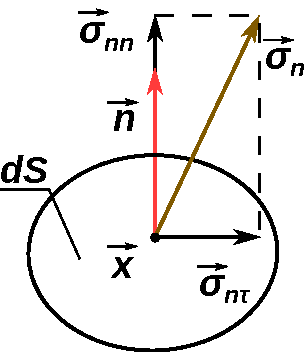
\includegraphics[width=0.7\textwidth]{../img/sigma_decomposition.pdf}
			
			\scriptsize
			Разложение напряжения на нормальную и тангенциальную составляющие
		\end{column}
		\begin{column}{0.6\textwidth}
			\begin{exampleblock}{Нормальная составляющая}
				\parbox{\textwidth}{
					\[
					\sigma_{nn} = n^i n^k \sigma_{ik} = (n^i)^2 \sigma_i
					\]				
				}
			\end{exampleblock}\pause
			\begin{exampleblock}{Тангенциальная составляющая}
				\parbox{\textwidth}{
					\[
					\sigma_{n\tau}^2 = \sigma_n^2-\sigma_{nn}^2  
%					\]
%					\[
					=   
					 n^i n^k \sigma_{il} \sigma_{ks} (g^{ls} - n^l n^s)
					=
					\]
					\[
					= n^i n^k \sigma_i \sigma_k (\delta^{ik} - n^i n^k)
					\]
				}
			\end{exampleblock}
			\begin{exampleblock}{Полное напряжение}
			\parbox{\textwidth}{
				\centering
				\[
				\vec{\sigma}_n^2 = 	(n^l \sigma_l \vec{g}_l) \cdot (n^k \sigma_k \vec{g}_k)= \sum_{k} (n^k \sigma_k)^2
%				n^l n^k \sigma^l \sigma^k g_{lk}.
				\]
			}
			\end{exampleblock}
			
		\end{column}
	\end{columns}

%	\parbox{\textwidth}{
%		\centering
%		Здесь $g_{lk} = \vec{g}_l \cdot \vec{g}_k$, $g^{lk} = \vec{g}^l \cdot \vec{g}^k$ -- метрические тензоры.
%	}

}

\frame{
	\frametitle{ Варианты напряженного состояния }
	
	\begin{exampleblock}{Определение}
		\parbox{\textwidth}{
			Если все три главных напряжения не равны нулю, то такое напряженное состояние называется \alert{трехосным}. Если одно из главных напряжений равно нулю, то такое напряженное состояние называется плоским, или \alert{двухосным}. Если два главных напряжения равны нулю, то такое напряженное состояние называется \alert{одноосным}.
			
		}
	\end{exampleblock}

	\begin{exampleblock}{Давление}
		\parbox{\textwidth}{
			
			Важной характеристикой тензора напряжений является давление, определяемое первым инвариантом тензора напряжений:
			\[
			p = -\frac{1}{3}(\sigma_{11}+\sigma_{22}+\sigma_{33})=-\frac{1}{3} \sigma_{kk}.
			\]
			
			Тензор напряжений часто записывают в виде суммы шаровой и девиаторной составляющих:
			\[
			\sigma_{ij} = -p\delta_{ij}+\tau_{ij}.
			\]
		
		}
	\end{exampleblock}

}

\frame{
	\frametitle{Обтекание покоящейся сферы идеальной жидкостью}
	
	\begin{exampleblock}{Выражение для давления}
	\parbox{\textwidth}{
		\[
		\frac{p(\theta)-p_\infty}{\rho} = \frac{V^2}{2}\left( 1- \frac{9}{4} \sin^2 \theta \right),\quad
		\sigma = -pI,
		\]
		где $p(\theta)$ -- давление жидкости на поверхности сферы; $p_\infty$ -- давление жидкости на бесконечности; $V$ -- скорость жидкости на бесконечности; $\rho$ -- плотность жидкости; $\theta$ -- полярный угол в сферической системе координат.
		
	}
	\end{exampleblock}

	\pause
	\begin{exampleblock}{Парадокс Даламбера}
	\parbox{\textwidth}{
		\medskip
		\[
		\vec{F} = -\int\limits_{S} n^i\sigma_i^j\vec{e}_j \, dS = 
		-\int\limits_{S} \left[\rho\frac{V^2}{2}\left( 1- \frac{9}{4} \sin^2 \theta \right) + p_\infty\right]  \vec{n}\, dS = 0.
		\]
		
	}
	\end{exampleblock}
}


\frame{
	\frametitle{Медленное обтекание покоящейся сферы вязкой жидкостью}
	
	\only<1>{

	\begin{exampleblock}{Компоненты тензора напряжений на поверхности сферы}
		\parbox{\textwidth}{
			\[
			\sigma = -pI + 2\mu e,
			\]
			где $p$ -- давление; $\mu$ -- вязкость жидкости; $e$ -- тензор скоростей деформаций.
			
			\smallskip
			В сферической системе координат ($r$, $\theta$, $\varphi$):
			\[
			\sigma_{rr}|_{r=a} = \left( -p + 2 \mu \pd{v_r}{r}\right)_{r=a} = \frac{3}{2}\mu\frac{U}{a}\cos\theta,\quad
			\sigma_{\varphi r}|_{r=a} = \sigma_{r \varphi}|_{r=a} = 0,
			\]	
			\[
			\sigma_{\theta r}|_{r=a} = \sigma_{r\theta}|_{r=a} = \mu\left(\frac{1}{r}\pd{v_r}{\theta}+\pd{v_\theta}{r} -\frac{v_\theta}{r} \right)_{r=a}=-\frac{3\mu U}{2a}\sin\theta,
			\]	
%			\[
%			
%			\]	
			где $v_r$, $v_\theta$ -- радиальная и полярная составляющие скорости; $a$ -- радиус сферы; $U$ -- скорость жидкости на бесконечности; $\theta$ -- полярный угол.
			
		}
	\end{exampleblock}
	}

	\only<2>{
	\begin{exampleblock}{Формула Стокса}
	\parbox{\textwidth}{
		\medskip
		\[
		W = \vec{F} \cdot \vec{e}_z = -\int\limits_{S} (n^i\sigma_i^j\vec{e}_j) \cdot \vec{e}_z \, dS = \int\limits_S (\sigma_{rr}\cos\theta - \sigma_{r\theta}\sin\theta) dS = 
		\]
		\[
		=
		\int\limits_0^\pi (\sigma_{rr}\cos\theta - \sigma_{r\theta}\sin\theta) 2 \pi a^2 \sin\theta d\theta = 
		3\pi\mu U a \int\limits_0^\pi \sin\theta d\theta =
		6\pi\mu U a,
		\]
		где $i,j \in \{r, \theta, \varphi\}$; $\vec{e}_z$ -- единичный вектор, направленный по направлению течения.
	}
	\end{exampleblock}
	}
}


\frame{
	\frametitle{ Литература }
	\parbox{\textwidth}{
	\begin{itemize}[label=]
		\item {\em Нигматулин Р.И.} Механика сплошной среды. Кинематика. Динамика. Термодинамика. Статистическая динамика. М.:ГЭОТАР-Медиа, 2014.
	\end{itemize}
	}
	
}


\end{document}
